\documentclass{sdkslides} 
\usepackage[T1]{fontenc}
\usepackage{graphicx}
\usepackage{amssymb,amsmath}
\usepackage{url}
\usepackage{lastpage}
\usepackage{epstopdf}
%\usepackage[pdfpagemode=None,colorlinks=true,urlcolor=red, linkcolor=black,citecolor=black,pdfstartview=FitH]{hyperref}
\usepackage{dirtree}
\usepackage{mdframed}
\usepackage[export]{adjustbox}
\usepackage{caption}
\usepackage{apacite}
\usepackage{tikz}
\usepackage{subfig}
\usetikzlibrary{positioning,shapes,shadows,arrows}
\tikzset{
  every overlay node/.style={
    %draw=black,fill=white,rounded corners,
    anchor=north west, inner sep=0pt,
  },
  thick/.style=      {line width=0.3mm},
}
\def\tikzoverlay{%
   \tikz[remember picture, overlay]\node[every overlay node]
}%

%%%% This for easy placemnet of figure inside a block
\newcommand{\putfig}[3][1.0]{
    \begin{block}{#3}
        \includegraphics[width=#1\linewidth,height=#1\textheight,keepaspectratio]{#2}
    \end{block}
}
%%%%

%%%% To insert lecture date
%\newcommand{\lectdate}{23.1.2020}
\newcommand{\lectdate}{\today}
%%%%
\newcommand{\sectname}{Section Name}

\title{\Huge{TheSyDeKick}\\ \vspace{0.2in} \normalsize{System development and
verification framework in Python}}

\author{Presenter: Marko Kosunen \\Authors: TheSyDeKick contributors}
\date{\lectdate}

\sdkfootertext{TheSyDeKick Roadshow}{\lectdate}{\arabic{page}/\pageref{LastPage}\ }

% Copies outline as an sectiontitleslide
%\AtBeginSection[]
%{
%    \begin{frame}{Outline}
%        \tableofcontents[currentsection]
%    \end{frame}
%}
\begin{document}

%%%%%%%%%%%%%%%%%%%%%%%%%%%%%%%%%%%%%%%%%%%%%%%%%%%%%%%%%%%%%%%%%%%%%%%%%%%%%
% Generates the titleframe
\section*{Title}
\sdktitleframe
%%%%%%%%%%%%%%%%%%%%%%%%%%%%%%%%%%%%%%%%%%%%%%%%%%%%%%%%%%%%%%%%%%%%%%%%%%%%%

%%%%%%%%%%%%%%%%%%%%%%%%%%%%%%%%%%%%%%%%%%
%%%% CONTENTS %%%%%%%%%%%%%%%%%%%%%%%%%%%%
%%%%%%%%%%%%%%%%%%%%%%%%%%%%%%%%%%%%%%%%%%
\section*{Outline}
\begin{frame}[c]
    \frametitle{Outline}
    \tableofcontents
\end{frame}

%%%%%%%%%%%%%%%%%%%%%%%%%%%%%%%%%%%%%%%%%%
%%%% SLIDES BEGIN HERE %%%%%%%%%%%%%%%%%%%
%%%%%%%%%%%%%%%%%%%%%%%%%%%%%%%%%%%%%%%%%%


%%%%%%%%%%%%%%%%%%%%%%%%%%%%%%%%%%%%%%%%%%%%%%%%%%%%%%%%%%%%%%%%%%%%%%%%%%%%%
\sectiontitle[TheSyDeKick - What it is]

%%%%%%%%%%%%%%%%%%%%%%%%%%%%%%%%%%%%%%%%%%
\renewcommand{\sectname}{What is TheSyDeKick}
\subsection*{\sectname}
\begin{frame}[t]
    \frametitle{\sectname}
    \begin{block}{TheSyDeKick at glance}
        \begin{center}
            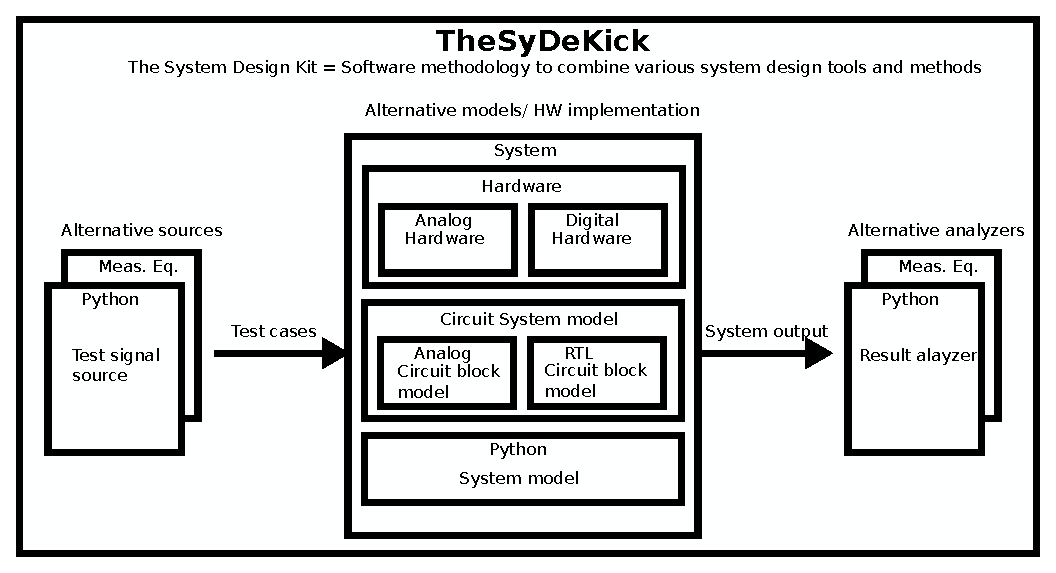
\includegraphics[width=0.75\textwidth]{Pics/TheSDK_block_diagram.eps}
        \end{center}
    \end{block}
    \begin{itemize}
        \item TheSyDeKick is a framework to enable programmatic
            verification of complex mixed signal systems. Contributed by
            multiple designers.
    \end{itemize}
\end{frame}

%%%%%%%%%%%%%%%%%%%%%%%%%%%%%%%%%%%%%%%%%%
\renewcommand{\sectname}{TheSyDeKick project structure}
\subsection*{\sectname}
\begin{frame}[t]
    \frametitle{\sectname}
    \begin{block}{TheSyDeKick project structure}
        \begin{center}
            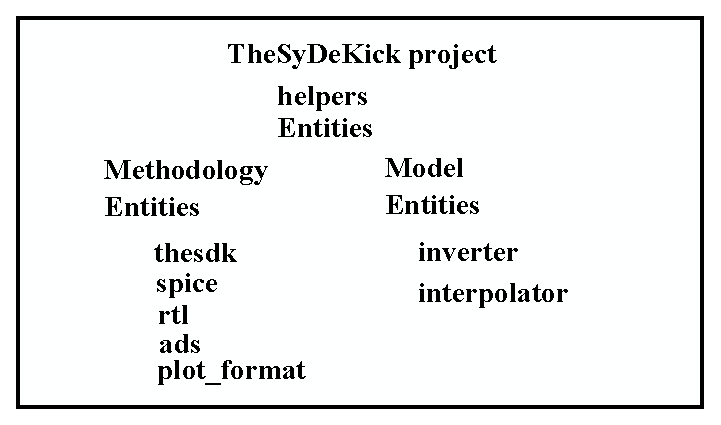
\includegraphics[width=0.5\textwidth]{Pics/TheSyDeKick-entity-principles.eps}
        \end{center}
    \end{block}
    \begin{itemize}
        \item TheSyDeKick is a well structured container for: 
            \begin{itemize}
                \item Python packages (Entities), that provide
                    \emph{formalism and methods to run simulations in
                    python, and with external simulators}
                \item Python packages (Entities), that provide
                    formalism to create and use \emph{IO compatible models}
            \end{itemize}
    \end{itemize}
\end{frame}

%%%%%%%%%%%%%%%%%%%%%%%%%%%%%%%%%%%%%%%%%%
\renewcommand{\sectname}{TheSyDeKick project structure}
\subsection*{\sectname}
\begin{frame}[t]
    \frametitle{\sectname}
    \begin{block}{TheSyDeKick project structure}
        \begin{center}
            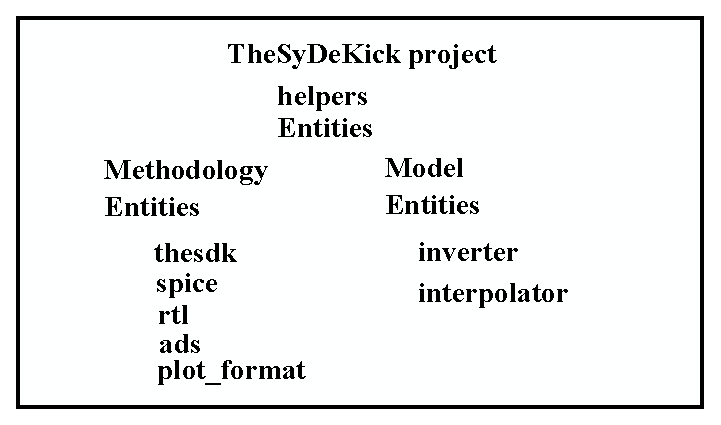
\includegraphics[width=0.5\textwidth]{Pics/TheSyDeKick-entity-principles.eps}
        \end{center}
    \end{block}
    \begin{itemize}
        \item TheSydeKick is a cumulative collection of Python classes and
            methods that help the designer to carry out the most common
            tasks encountered in microelectronics design. Most likely the
            \emph{simulation task you have in mind has some supporting
            methodology available in TheSyDeKick}
    \end{itemize}
\end{frame}

%%%%%%%%%%%%%%%%%%%%%%%%%%%%%%%%%%%%%%%%%%
\renewcommand{\sectname}{TheSyDeKick project structure}
\subsection*{\sectname}
\begin{frame}[t]
    \frametitle{\sectname}
    \begin{block}{TheSyDeKick project structure}
        \begin{center}
            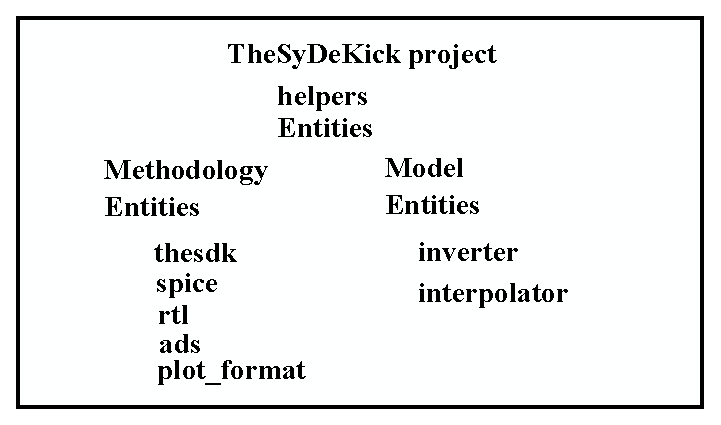
\includegraphics[width=0.5\textwidth]{Pics/TheSyDeKick-entity-principles.eps}
        \end{center}
    \end{block}
    \begin{itemize}
       \item TheSyDeKick formalism helps the designer to: 
        \begin{itemize}
            \item Write and simulate modular, hierarchical, IO compatible
                hardware models with various levels of abstraction (python,
                spice/RTL or even EM field simulator)
            \item Control the abstraction level with one parameter on
                chosen level of hierarchy.
        \end{itemize}
        \item TheSyDeKick is \emph{nothing more}
    \end{itemize}
        {\tiny
        \url{https://github.com/TheSystemDevelopmentKit/thesdk_template/wiki/The-System-Development-Kit}}
\end{frame}


%%%%%%%%%%%%%%%%%%%%%%%%%%%%%%%%%%%%%%%%%%
\renewcommand{\sectname}{How it is constructed?}
\subsection*{\sectname}
\begin{frame}[t]
    \frametitle{\sectname}
    \begin{itemize}
        \item Minimum set of structural constraints, 
            \begin{itemize}
                \item IO definitions
                \item Blocks described as connected \emph{Entities}.
            \end{itemize}
        \item Aims to automation of \emph{repetitive, well structured tasks}
            \begin{itemize}
                \item Model and modeling environment structure with init scripts
                \item Running simulations
                \item Defining simulator calls
                \item Documentation with Docstrings see for
                    example. {\tiny
                    \url{https://thesystemdevelopmentkit.github.io/docs/index.html}}
            \end{itemize}
        \item Currently supports Python, Verilog, VHDL and three Spice
            variants.
        \item Open source simulators: Icarus and Verilator, for Verilog, GHDL
            for VHDL, NgSpice for analog
            circuits.
        \item Under construction: Measurement equipment.
    \end{itemize}
    {\tiny \url{https://github.com/TheSystemDevelopmentKit}}
\end{frame}

%%%%%%%%%%%%%%%%%%%%%%%%%%%%%%%%%%%%%%%%%%
\renewcommand{\sectionname}{TheSyDeKick project file structure}
\subsection*{\sectionname}
\begin{frame}[t]
    \frametitle{\sectionname}
    \begin{block}{TheSyDeKick project structure}
    \begin{minipage}[t]{0.3\textwidth}
    \parbox{\textwidth}{
        \dirtree{% 
            .1 thesydekick\_project/.
            .2 Entities/.
            .3 thesdk/.
            .3 rtl/.
            .3 spice/.
            .3 ads/.
            .3 amplifier/.
            .4 amplifier/.
            .5 \_\_init\_\_.py.
            .4 spice/.
            .4 simulations/.
            .4 doc/.
        }
    }
    \end{minipage}
    \end{block}
    {\tiny \url{https://github.com/TheSystemDevelopmentKit/thesdk_template}}
\end{frame}


%%%%%%%%%%%%%%%%%%%%%%%%%%%%%%%%%%%%%%%%%%%%%%%%%%%%%%%%%%%%%%%%%%%%%%%%%%%%%
\sectiontitle[Simulator interfaces]

%%%%%%%%%%%%%%%%%%%%%%%%%%%%%%%%%%%%%%%%%%%%%%%%%%%%%%%%%%%%%%%%%%%%%%%%%%
\renewcommand{\sectname}{Analog simulator interface}
\subsection*{\sectname}
\begin{frame}[t]
    \frametitle{\sectname}
    \begin{itemize}
        \item Calling analog simulators is handled through a common interface, the \textbf{spice} module
        \item Ultimate goal of \textbf{spice}: support for most industry standard simulators
        \begin{itemize}
            \item General (w.r.t to simulator), reusable simulation testbenches
            \item Centralized post processing based on open source tools and
                libraries.
        \end{itemize}
            \item Save time in re-writing testbenches for different simulations and centralize effort to all-in-one testbench
        \begin{itemize}
        \item Currently support for DC, AC, and Transient analysis. Easy to
            add other analysis types as IO formats are the same. 
        \end{itemize}
    \end{itemize}
    {\tiny \url{https://github.com/TheSystemDevelopmentKit/spice}}
\end{frame}

%%%%%%%%%%%%%%%%%%%%%%%%%%%%%%%%%%%%%%%%%%%%%%%%%%%%%%%%%%%%%%%%%%%%%%%%%%%%%
\renewcommand{\sectname}{Digital simulator interface}
\subsection*{\sectname}
\begin{frame}[t]
    \frametitle{\sectname}
    \begin{itemize}
        \item Calling digital simulators is handled the \textbf{rtl} module
        \begin{itemize}
            \item Most commonly used simulation testbenches automatically
                generated for both Verilog and VHDL design under tests.
            \item Automated file IO generation for strings (bit vectors), integers, and complex numbers. 
            \item Support for any signal type through customizable format
                parameter.
        \end{itemize}
        %\begin{itemize}
        %    \item Future plans: Support for Verilator
        %\end{itemize}
    \end{itemize}
    {\tiny   \url{https://github.com/TheSystemDevelopmentKit/rtl}}
\end{frame}

%%%%%%%%%%%%%%%%%%%%%%%%%%%%%%%%%%%%%%%%%%
\renewcommand{\sectionname}{EM field simulator interface}
\subsection*{\sectionname}
\begin{frame}[t]
    \frametitle{\sectionname}
    \begin{itemize}
        \item Interface entity \textbf{ads} enables EM simulator Momentum from python desing
            environment.
        \item Used so far for example:
            \begin{itemize}
                \item Together with Berkeley Analog Generator in
                    characterization of parametrized inductors transformers.
                \item In extraction of S-parameters from 3D layout structures.
            \end{itemize}
    \end{itemize}
    { \tiny \url{https://github.com/TheSystemDevelopmentKit/ads}}
\end{frame}
%%%%%%%%%%%%%%%%%%%%%%%%%%%%%%%%%%%%%%%%%%%%%%%%%%%%%%%%%%%%%%%%%%%%%%%%%%%%%
\renewcommand{\sectname}{TheSyDeKick simulation procedure}
\begin{frame}[t]
    \frametitle{\sectname}
        \begin{enumerate}
            \item Write the testbench
            \begin{enumerate}
                \item Specify analysis type, inputs, outputs, supplies etc. based on TB properties
                \item Configure simulator options, corners, etc. based on
                    testbench properties
                \item Specify desired outputs, e.g. FFT of waveform, transient waveform
                \item Specify run cases, e.g. transient analysis for 2 different netlists, etc.
            \end{enumerate}
            \item Run the simulation
            \item Analyze results
            \item (Optional) Repeat simulation for different sets of parameters
        \end{enumerate}
        \begin{itemize}
            \item Once you have one testbench, reuse for similar applications makes things faster
            \item Results saved (if user chooses so), no need to repeat lengthy simulations to fix errors in post processing
        \end{itemize}
\end{frame}

%%%%%%%%%%%%%%%%%%%%%%%%%%%%%%%%%%%%%%%%%%%%%%%%%%%%%%%%%%%%%%%%%%%%%%%%%%%%%
\sectiontitle[Principle of simulation]

%%%%%%%%%%%%%%%%%%%%%%%%%%%%%%%%%%%%%%%%%%%%%%%%%%%%%%%%%%%%%%%%%%%%%%%%%%%%%
\renewcommand{\sectionname}{First step: Self test }
\subsection*{\sectionname}
\begin{frame}[t]
    \frametitle{\sectionname}
    \begin{center}
        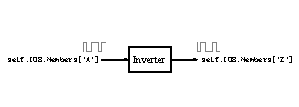
\includegraphics[width=0.95\textwidth]{Pics/inverter_single_1}
    \end{center}
    \begin{itemize}
        \item Example: inverter
        \item Functional model: Inverts input signal
        \item IOS is a Bundle-type container for storing IO data
        \item Can have as many members as needed
    \end{itemize}
\end{frame}

%%%%%%%%%%%%%%%%%%%%%%%%%%%%%%%%%%%%%%%%%%%%%%%%%%%%%%%%%%%%%%%%%%%%%%%%%%%%%
\begin{frame}[t]
    \frametitle{\sectionname}
    \begin{center}
        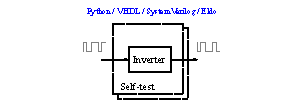
\includegraphics[width=0.95\textwidth]{Pics/inverter_single_2}
    \end{center}
    \begin{itemize}
        \item Multiple models for the same entity: Python,spice,rtl
        \item Self-test is a way to verify the functionality of entity ``in
            vacuum''
        \item Self-test generates and feeds the identical input
            data to all simulators
    \end{itemize}
\end{frame}

%%%%%%%%%%%%%%%%%%%%%%%%%%%%%%%%%%%%%%%%%%%%%%%%%%%%%%%%%%%%%%%%%%%%%%%%%%%%%
\renewcommand{\sectionname}{Next step: Connecting Entities}
\subsection*{\sectionname}
\begin{frame}[t]
    \frametitle{\sectionname}
    \begin{center}
        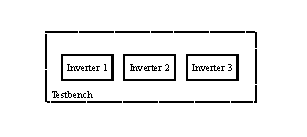
\includegraphics[width=0.95\textwidth]{Pics/inverter_chain_0}
    \end{center}
    \begin{itemize}
        \item Entities care connected inside another entities, (or in a
            testbench).
        \item Chain of inverter instances can created with a for loop.
    \end{itemize}
\end{frame}

%%%%%%%%%%%%%%%%%%%%%%%%%%%%%%%%%%%%%%%%%%%%%%%%%%%%%%%%%%%%%%%%%%%%%%%%%%%%%
\begin{frame}[t]
    \frametitle{\sectionname}
    \begin{center}
        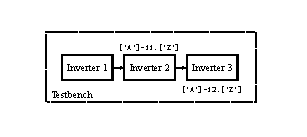
\includegraphics[width=0.95\textwidth]{Pics/inverter_chain_2}
    \end{center}
    \begin{itemize}
        \item Entities care connected inside another entities, (or in a
            testbench).
        \item Chain of inverter instances can created with a for loop.
        \item Data flow defined by IOS connections
    \end{itemize}
\end{frame}


%%%%%%%%%%%%%%%%%%%%%%%%%%%%%%%%%%%%%%%%%%%%%%%%%%%%%%%%%%%%%%%%%%%%%%%%%%%%%
\begin{frame}[t]
    \frametitle{\sectionname}
    \begin{center}
        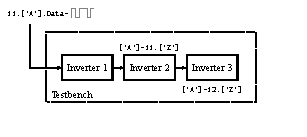
\includegraphics[width=0.95\textwidth]{Pics/inverter_chain_3}
    \end{center}
    \begin{itemize}
        \item Entities care connected inside another entities, (or in a
            testbench).
        \item Chain of inverter instances can created with a for loop.
        \item Data flow defined by IOS connections
        \item Signal is assigned as input of 1st element
    \end{itemize}
\end{frame}

%%%%%%%%%%%%%%%%%%%%%%%%%%%%%%%%%%%%%%%%%%%%%%%%%%%%%%%%%%%%%%%%%%%%%%%%%%%%%
\begin{frame}[t]
    \frametitle{\sectionname}
    \begin{center}
        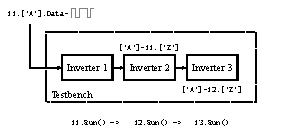
\includegraphics[width=0.95\textwidth]{Pics/inverter_chain_4}
    \end{center}
    \begin{itemize}
        \item Entities care connected inside another entities, (or in a
            testbench).
        \item Chain of inverter instances can created with a for loop.
        \item Data flow defined by IOS connections
        \item Signal is assigned as input of 1st element
        \item Signal is propagated through the chain by running the entities
            in user defined sequence
    \end{itemize}
\end{frame}

%%%%%%%%%%%%%%%%%%%%%%%%%%%%%%%%%%%%%%%%%%%%%%%%%%%%%%%%%%%%%%%%%%%%%%%%%%%%%
\begin{frame}[t]
    \frametitle{\sectionname}
    \begin{center}
        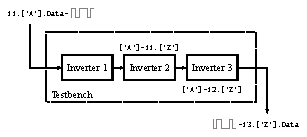
\includegraphics[width=0.95\textwidth]{Pics/inverter_chain_5}
    \end{center}
    \begin{itemize}
        \item In the end, the output of the last element contains processed data
    \end{itemize}
\end{frame}

%%%%%%%%%%%%%%%%%%%%%%%%%%%%%%%%%%%%%%%%%%%%%%%%%%%%%%%%%%%%%%%%%%%%%%%%%%
\sectiontitle[Example 1: Inverter tests]

%%%%%%%%%%%%%%%%%%%%%%%%%%%%%%%%%%%%%%%%%%
\renewcommand{\sectionname}{Verifying inverter system}
\subsection*{\sectionname}
\begin{frame}[t]
    \frametitle{\sectionname}
    \begin{itemize}
        \item Example of test hierarchy from bottom up: inverter, inverter
            testbench and inverter tests. 
    \end{itemize}
    \begin{block}{Inverter system serial test configuration}
        \begin{center}
            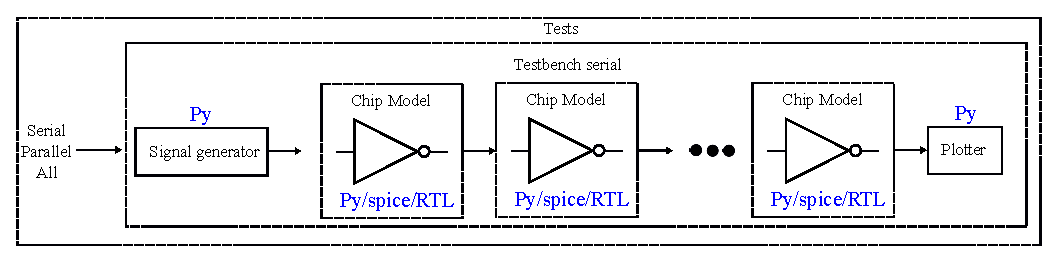
\includegraphics[width=\textwidth]{./Pics/Inverter_chain.eps}
        \end{center}
    \end{block}
\end{frame}

%%%%%%%%%%%%%%%%%%%%%%%%%%%%%%%%%%%%%%%%%%
\renewcommand{\sectionname}{Multiple testbench configurations}
\subsection*{\sectionname}
\begin{frame}[t]
    \frametitle{\sectionname}
    \begin{itemize}
        \item Construction methods of testbench class enable various test
            configurations.
        \item All parallel executions can be executed in parallel threads resulting in remarkable speedup. 
    \end{itemize}
    \begin{block}{Inverter system parallel test configuration}
        \begin{center}
            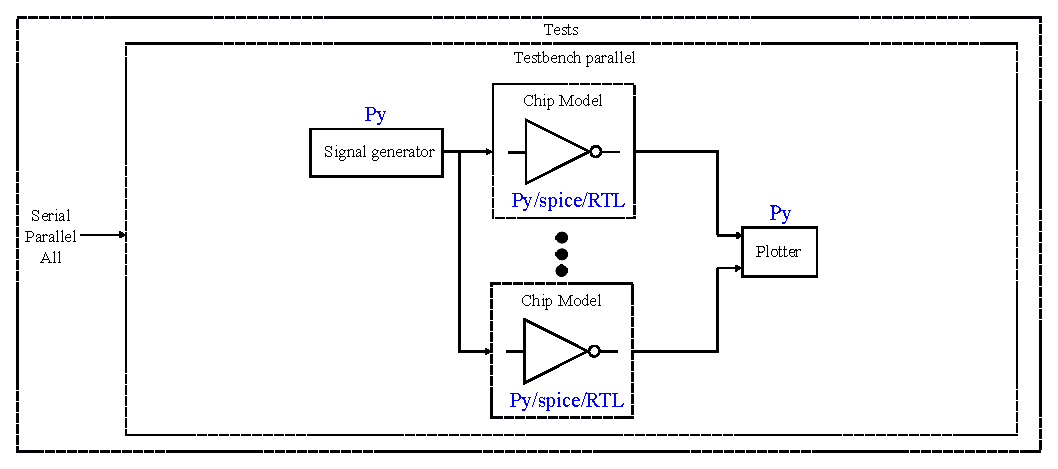
\includegraphics[width=\textwidth]{./Pics/Inverter_parallel.eps}
        \end{center}
    \end{block}
\end{frame}

%%%%%%%%%%%%%%%%%%%%%%%%%%%%%%%%%%%%%%%%%%
\renewcommand{\sectionname}{Inverter system verification results}
\subsection*{\sectionname}
\begin{frame}[t]
    \frametitle{\sectionname}
    \begin{block}{Inverter system results}
        \begin{center}
            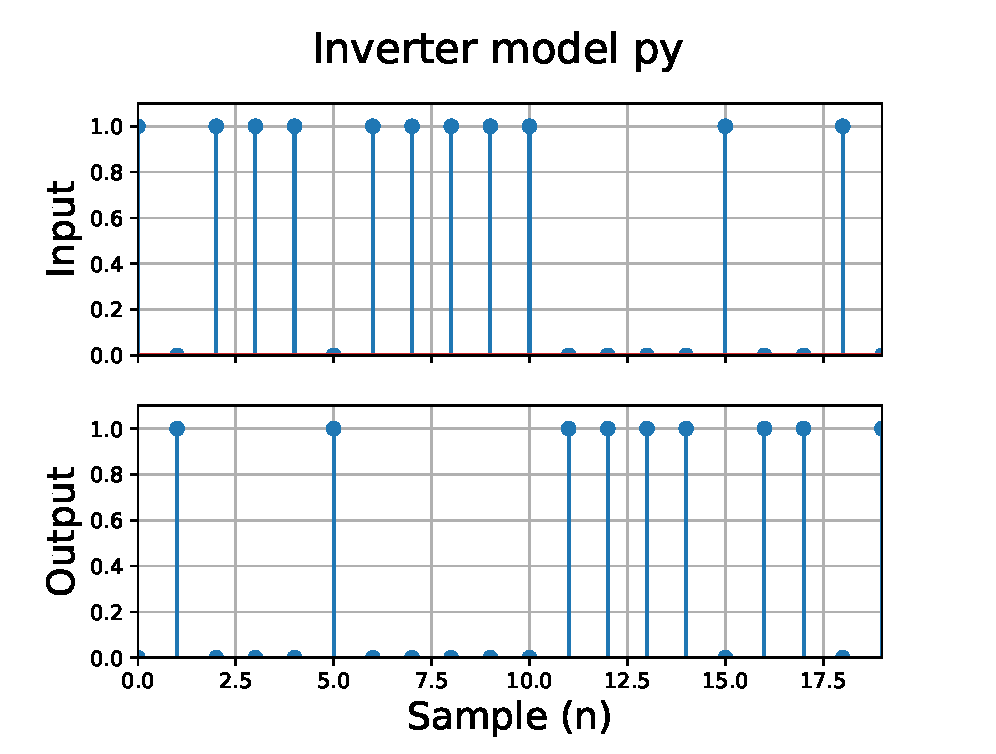
\includegraphics[width=0.3\textwidth]{./Pics/inv_serialpy.eps}
            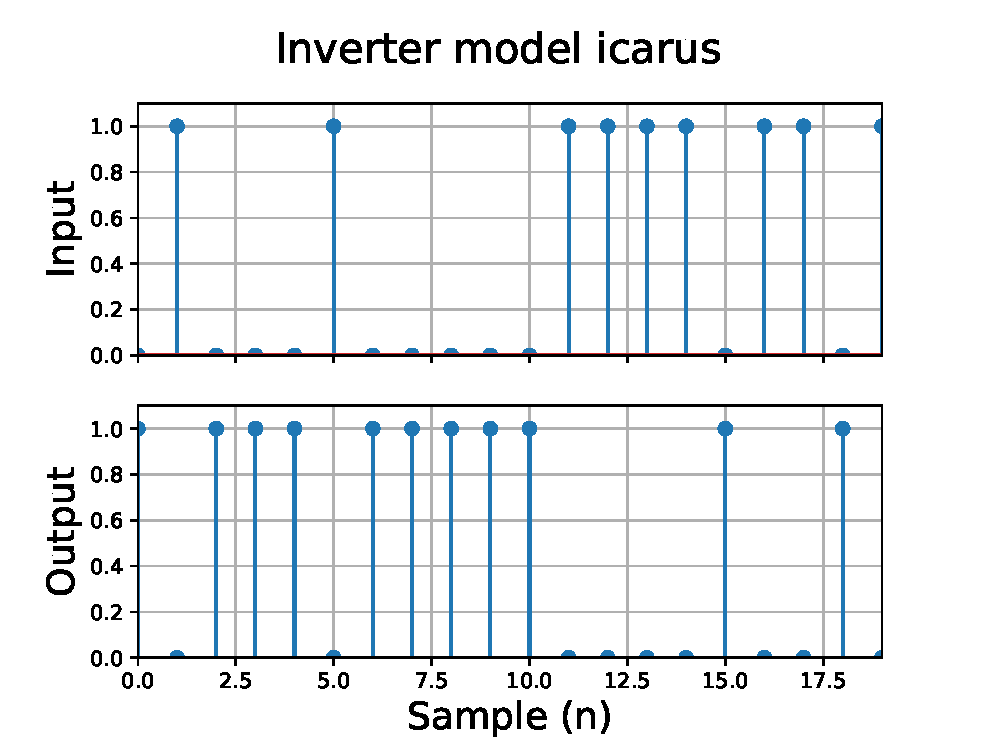
\includegraphics[width=0.3\textwidth]{./Pics/inv_serialicarus.eps}
            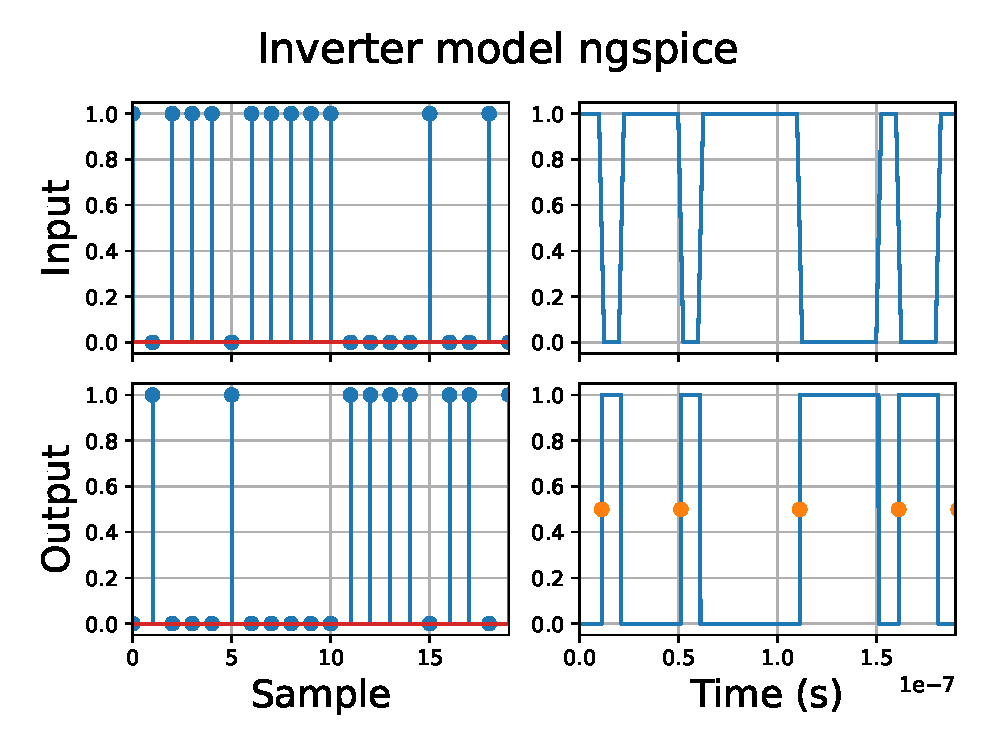
\includegraphics[width=0.3\textwidth]{./Pics/inv_serialngspice.eps}

            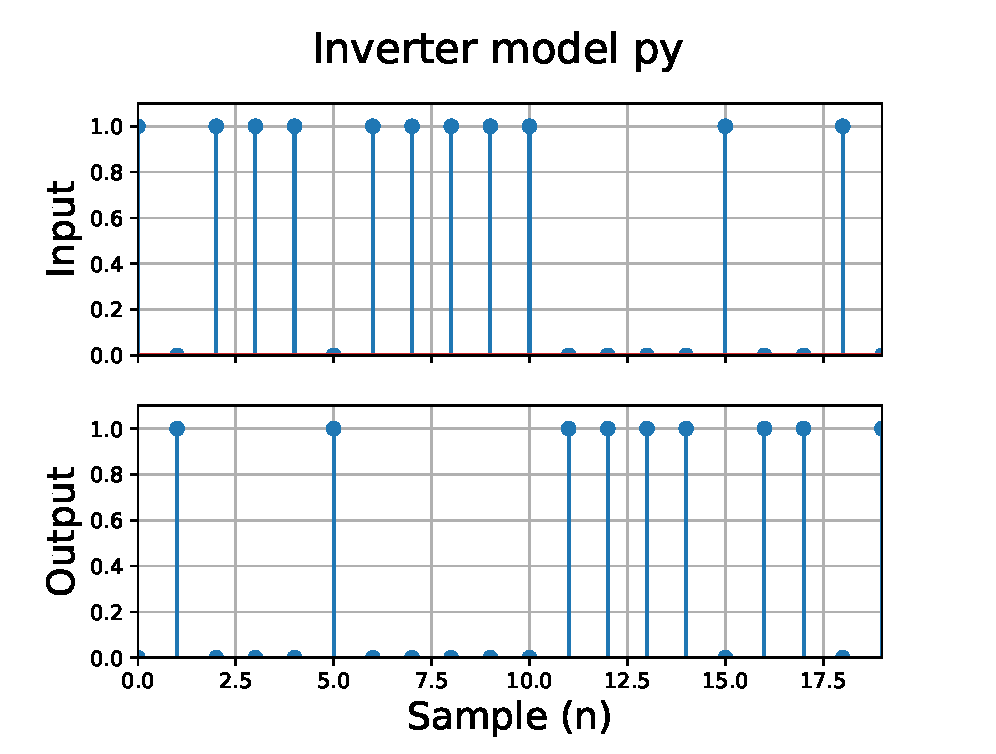
\includegraphics[width=0.3\textwidth]{./Pics/inv_serialpy.eps}
            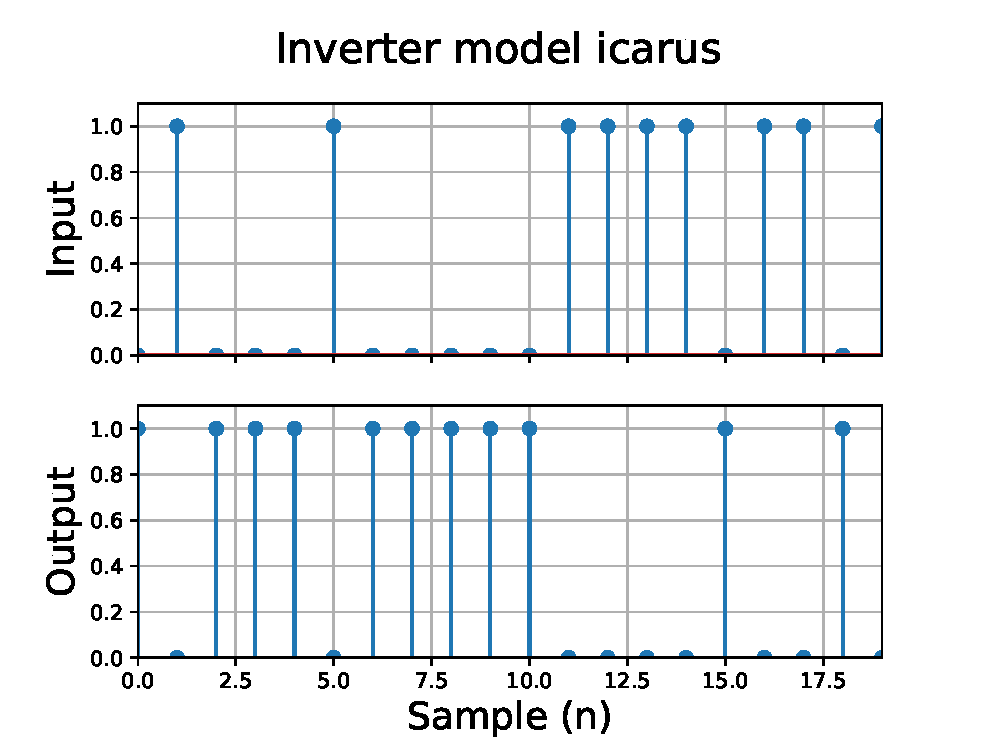
\includegraphics[width=0.3\textwidth]{./Pics/inv_serialicarus.eps}
            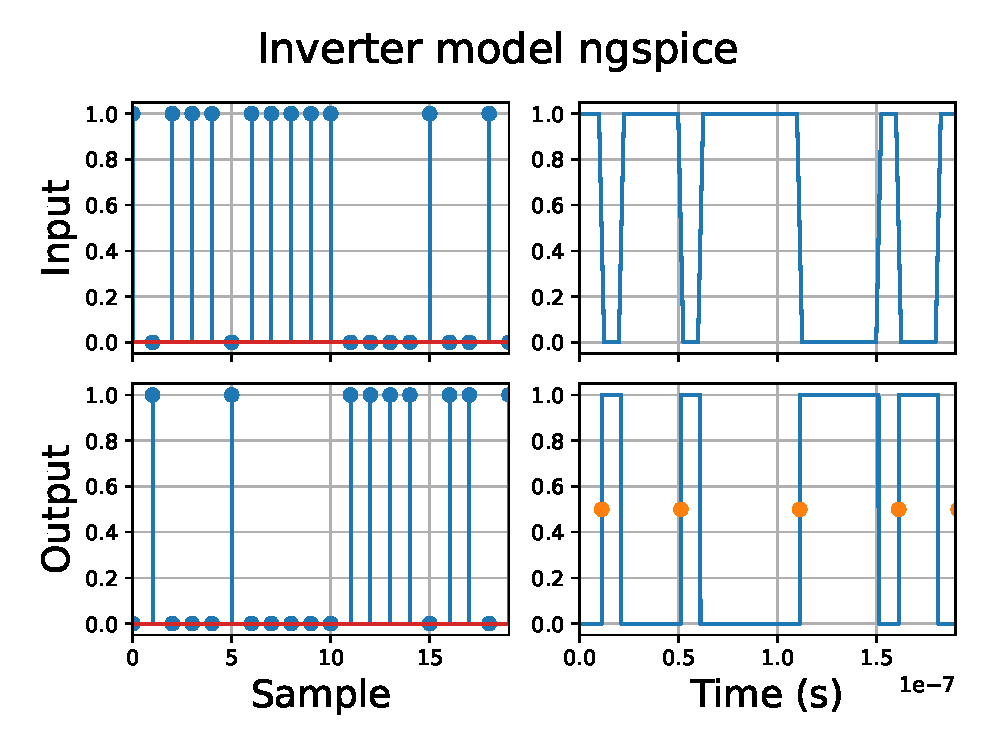
\includegraphics[width=0.3\textwidth]{./Pics/inv_serialngspice.eps}
        \end{center}
    \end{block}
\end{frame}



%%%%%%%%%%%%%%%%%%%%%%%%%%%%%%%%%%%%%%%%%%%%%%%%%%%%%%%%%%%%%%%%%%%%%%%%%%
\sectiontitle[Example 3: ADC model]

%%%%%%%%%%%%%%%%%%%%%%%%%%%%%%%%%%%%%%%%%%%%%%%%%%%%%%%%%%%%%%%%%%%%%%%%%%%%%
\renewcommand{\sectionname}{Example 3: ADC Model}
\subsection*{\sectionname} 
\begin{frame}[c]
    \frametitle{\sectionname}
    \begin{center}
        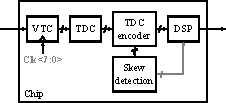
\includegraphics[width=0.9\textwidth]{Pics/sdk_model_0}
    \end{center}
\end{frame}

%%%%%%%%%%%%%%%%%%%%%%%%%%%%%%%%%%%%%%%%%%%%%%%%%%%%%%%%%%%%%%%%%%%%%%%%%%%%%
\renewcommand{\sectionname}{Example 3: ADC Model}
\subsection*{\sectionname} 
\begin{frame}[c]
    \frametitle{\sectionname}
    \begin{center}
        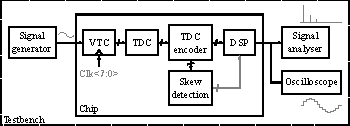
\includegraphics[width=0.9\textwidth]{Pics/sdk_model_1}
    \end{center}
\end{frame}

%%%%%%%%%%%%%%%%%%%%%%%%%%%%%%%%%%%%%%%%%%%%%%%%%%%%%%%%%%%%%%%%%%%%%%%%%%%%%
\renewcommand{\sectionname}{Example 3: ADC Model}
\subsection*{\sectionname} 
\begin{frame}[c]
    \frametitle{\sectionname}
    \begin{center}
        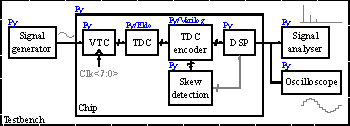
\includegraphics[width=0.9\textwidth]{Pics/sdk_model_2}
    \end{center}
\end{frame}

%%%%%%%%%%%%%%%%%%%%%%%%%%%%%%%%%%%%%%%%%%%%%%%%%%%%%%%%%%%%%%%%%%%%%%%%%%%%%
\renewcommand{\sectionname}{Example 3: ADC Model}
\subsection*{\sectionname} 
\begin{frame}[c]
    \frametitle{\sectionname}
    \begin{center}
        Full ADC Model in Python
        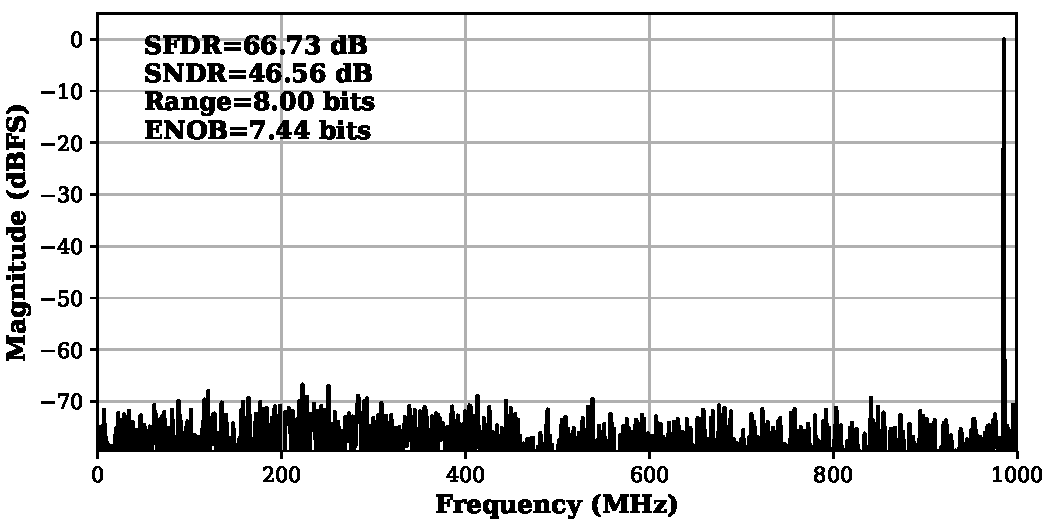
\includegraphics[width=0.8\textwidth]{Pics/latido_fft_py}
    \end{center}
    \begin{itemize}
        \item Spectrum plotted by signal\_analyser -module, which also
            calculates SNDR etc.
    \end{itemize}
\end{frame}

%%%%%%%%%%%%%%%%%%%%%%%%%%%%%%%%%%%%%%%%%%%%%%%%%%%%%%%%%%%%%%%%%%%%%%%%%%%%%
\renewcommand{\sectionname}{Example 3: ADC Model}
\subsection*{\sectionname} 
\begin{frame}[c]
    \frametitle{\sectionname}
    \begin{center}
        Full ADC Model in Python with Transistor-level TDC Model
        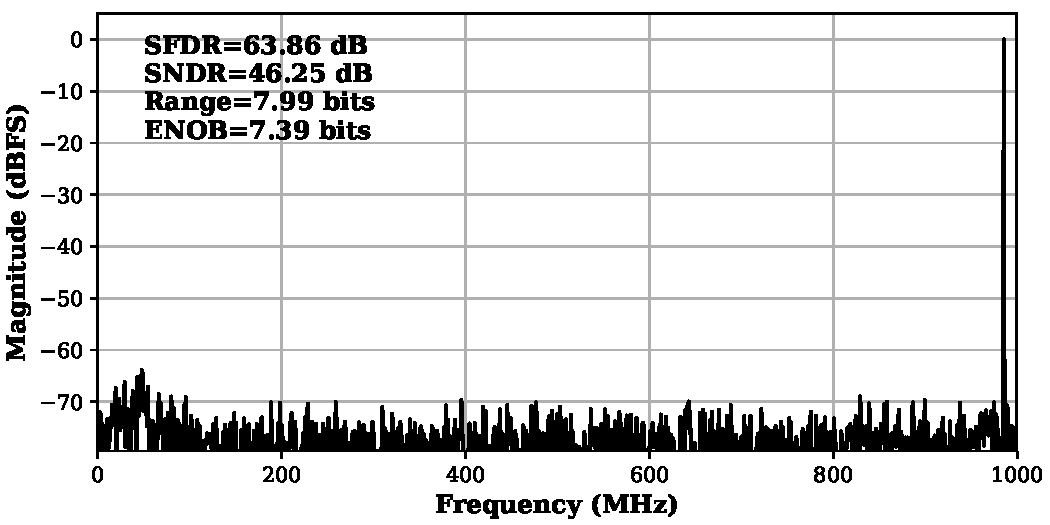
\includegraphics[width=0.8\textwidth]{Pics/latido_fft_eldo}
    \end{center}
    \begin{itemize}
        \item Same exact simulation as before, except the TDC block is
            simulated as a spice-netlist in Eldo
    \end{itemize}
\end{frame}

%%%%%%%%%%%%%%%%%%%%%%%%%%%%%%%%%%%%%%%%%%%%%%%%%%%%%%%%%%%%%%%%%%%%%%%%%%
\sectiontitle[Example 4: Multi-user MIMO receiver]

%%%%%%%%%%%%%%%%%%%%%%%%%%%%%%%%%%%%%%%%%%
\renewcommand{\sectionname}{Example 4: Multi-user MIMO receiver}
\subsection*{\sectionname}
\begin{frame}[t]
    \frametitle{\sectionname}
    \begin{center}
        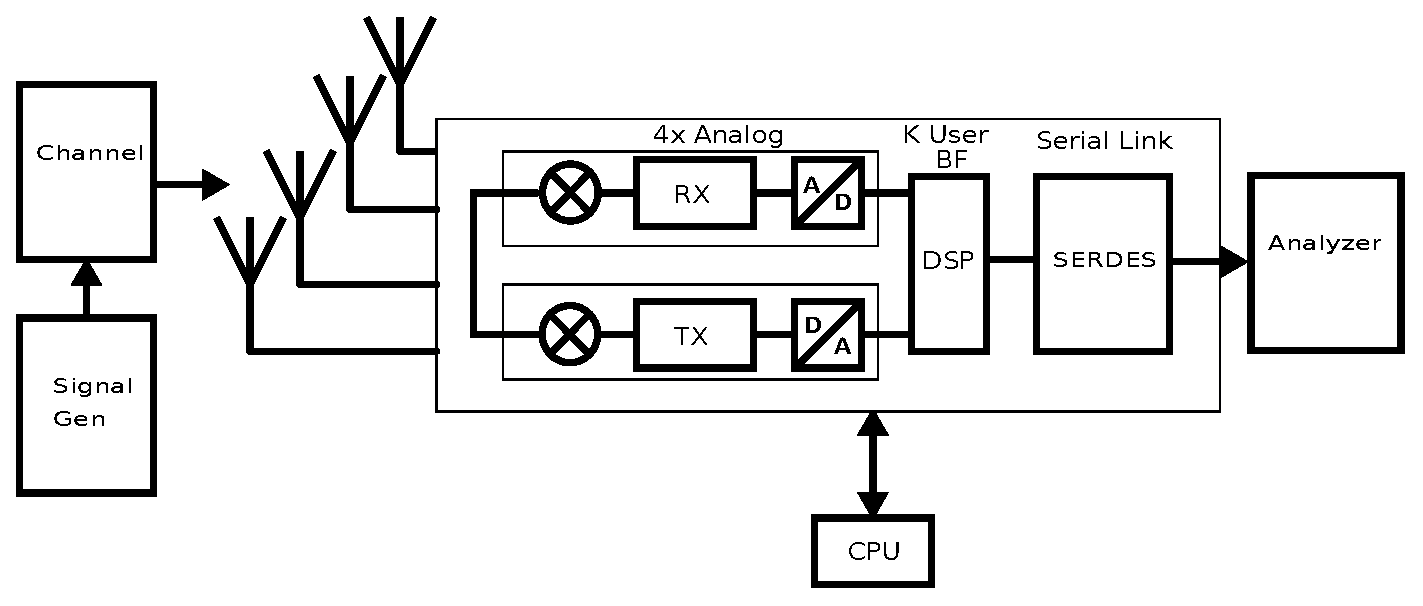
\includegraphics[width=\textwidth]{Pics/Fader2_simulator.eps}
    \end{center}
    \begin{itemize}
        \item Goals:
            \begin{itemize}
                \item  First, model the receiver of a single chip with python
                \item  Python models swappable to RTL and analog models 
                \item  Generated sub-blocks verified at the system level
                \item  Control the HW generators of the block (emerging feature)
            \end{itemize}

    \end{itemize}
\end{frame}
%%%%%%%%%%%%%%%%%%%%%%%%%%%%%%%%%%%%%%%%%%
\renewcommand{\sectionname}{DSP modeling example}
\subsection*{\sectionname}
\begin{frame}[c]
    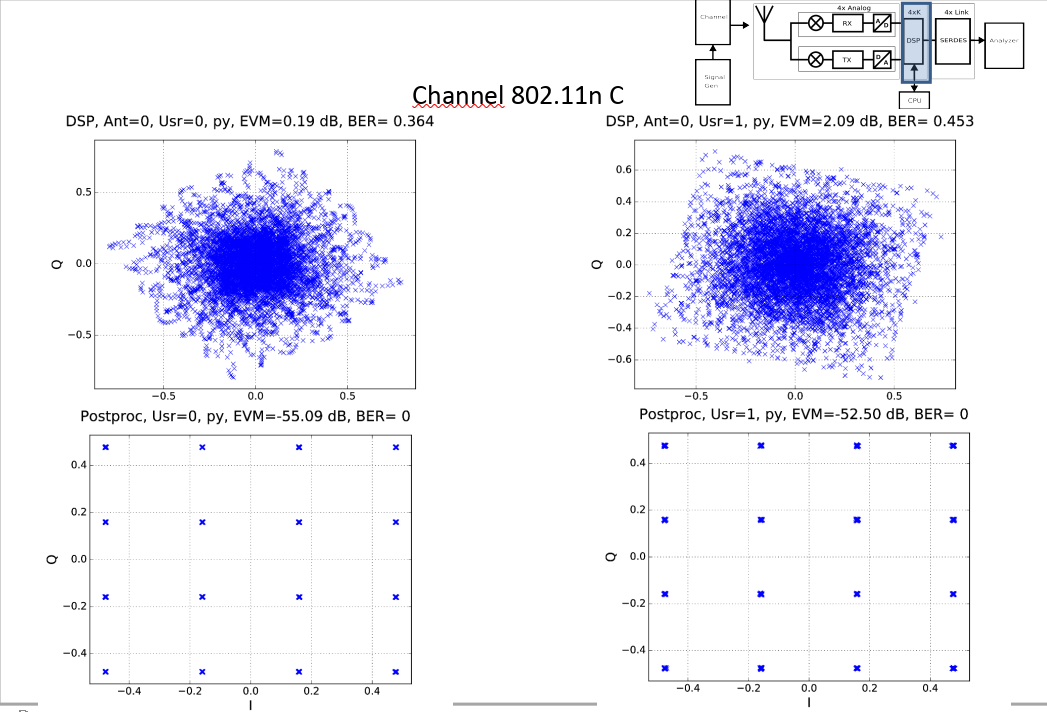
\includegraphics[width=\textwidth]{Pics/DSP-example-fader2-ideal.png}
\end{frame}

%%%%%%%%%%%%%%%%%%%%%%%%%%%%%%%%%%%%%%%%%%
\renewcommand{\sectionname}{Python/RTL example simulation}
\subsection*{\sectionname}
\begin{frame}[c]
    \begin{center}
        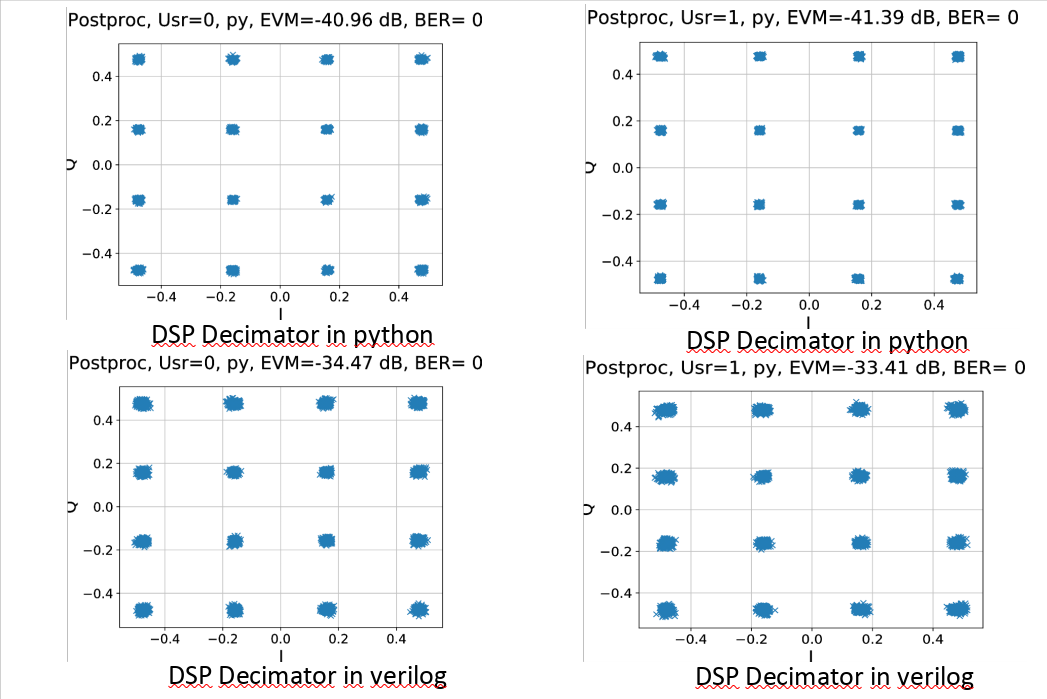
\includegraphics[width=\textwidth]{Pics/DSP-example-fader2-decimator_effect.png}
    \end{center}
\end{frame}

%%%%%%%%%%%%%%%%%%%%%%%%%%%%%%%%%%%%%%%%%%%%%%%%%%%%%%%%%%%%%%%%%%%%%%%%%%
\sectiontitle[Example 5: Outphasing transmitter]

%%%%%%%%%%%%%%%%%%%%%%%%%%%%%%%%%%%%%%%%%%
\renewcommand{\sectionname}{Outphasing transmitter system}
\subsection*{\sectionname}
\begin{frame}[c]
    \frametitle{\sectionname}
    \begin{block}{Outphasing system simulation}
        \begin{center}
            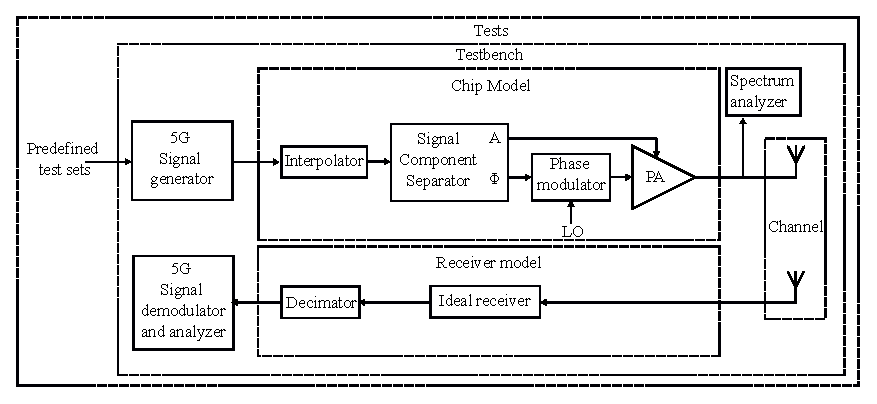
\includegraphics[width=\textwidth]{Pics/outphasing_model.eps}
        \end{center}
    \end{block}    \begin{itemize}
        \item System development
            \begin{itemize}
                \item  Model the transmitter chip with python
                \item  Model the ideal receiver in python
                \item  Simulate the functionality
            \end{itemize}
    \end{itemize}
\end{frame}

%%%%%%%%%%%%%%%%%%%%%%%%%%%%%%%%%%%%%%%%%%%
\begin{frame}[t]
    \frametitle{Interpolator frequency response}
    \begin{center}
        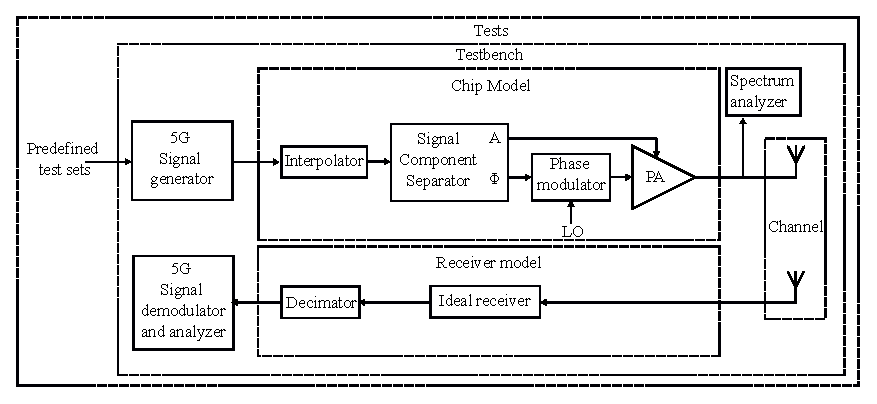
\includegraphics[width=0.5\textwidth]{Pics/outphasing_model.eps}
    \end{center}
    \begin{figure}
        \begin{center}
            \subfloat[Interpolator SW]{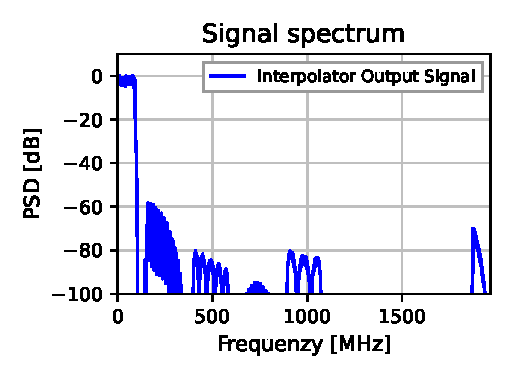
\includegraphics[width=0.4\textwidth]{./Pics/interp_out_f_sw.eps}}\qquad
            \subfloat[Interpolator
            HW]{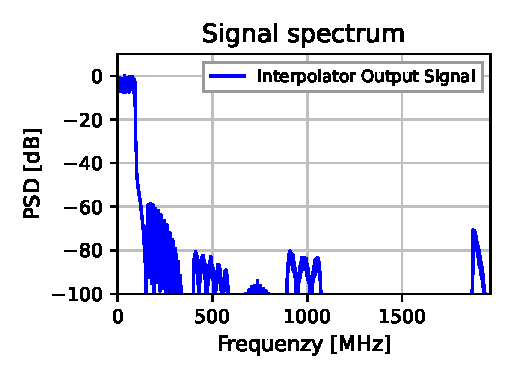
\includegraphics[width=0.4\textwidth]{./Pics/interp_out_f_hw.eps}}
        \end{center}
    \end{figure}

\end{frame}

%%%%%%%%%%%%%%%%%%%%%%%%%%%%%%%%%%%%%%%%%%
\begin{frame}[t]
    \frametitle{Interpolator EVM simulation}
    \begin{center}
        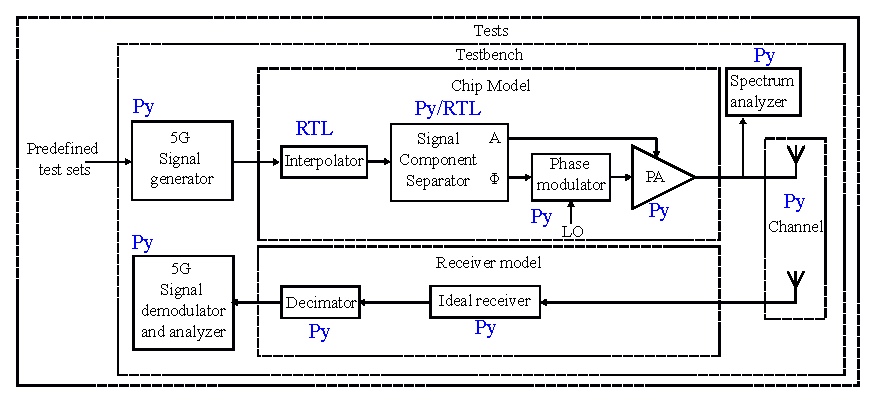
\includegraphics[width=0.5\textwidth]{Pics/outphasing_model_interp.eps}
    \end{center}
    \begin{figure}
        \begin{center}
            \subfloat[Interpolator HW (EVM,
            16-bit)]{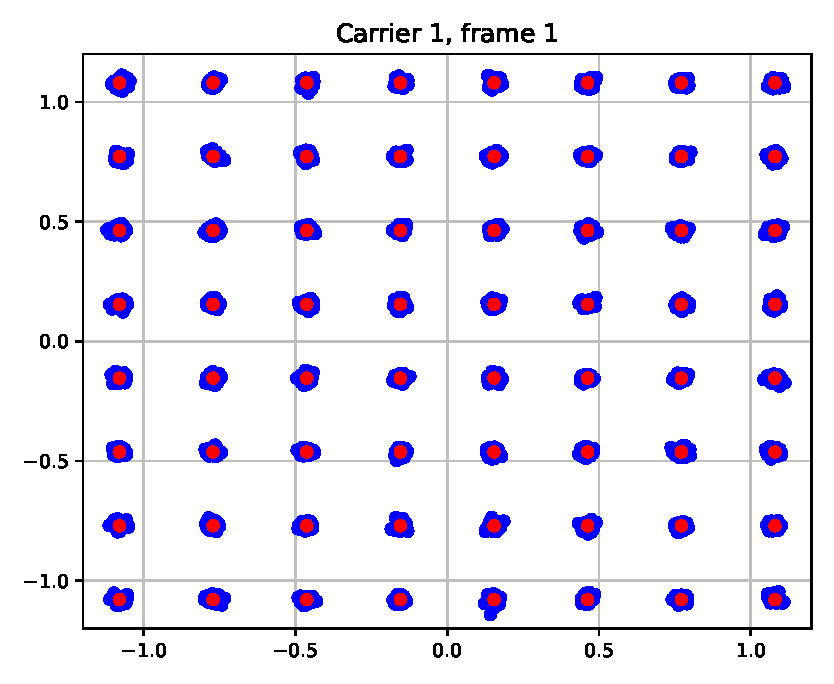
\includegraphics[width=0.30\textwidth]{Pics/evm_16bit.eps}}\qquad
            \subfloat[Interpolator HW (EVM,
            20-bit)]{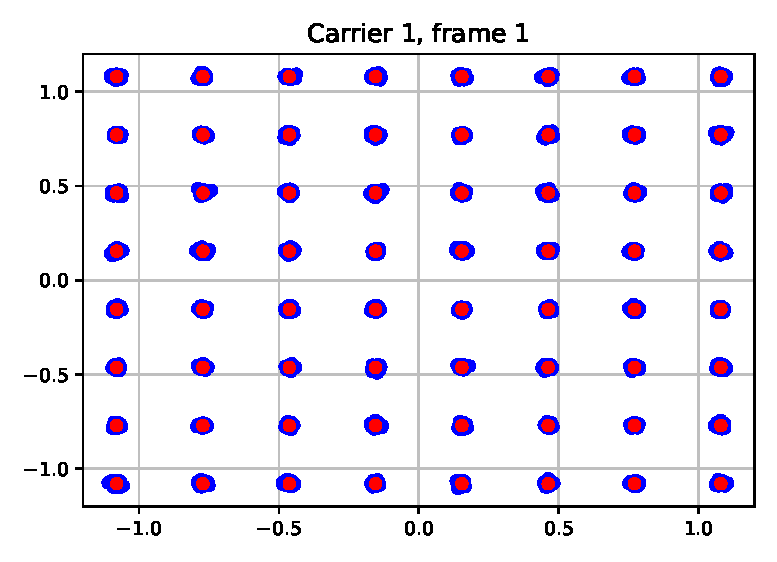
\includegraphics[width=0.4\textwidth]{Pics/evm_20bit.eps}}
        \end{center}
     \end{figure}
     \begin{itemize}
         \item EVM(16-bit): 1.6 - 1.52\%
         \item EVM(20-bit): 1.3 - 1.08\%
     \end{itemize}
\end{frame}

%%%%%%%%%%%%%%%%%%%%%%%%%%%%%%%%%%%%%%%%%%%
\begin{frame}[t]
    \frametitle{Interpolator EVM and ACLR}
    \begin{center}
        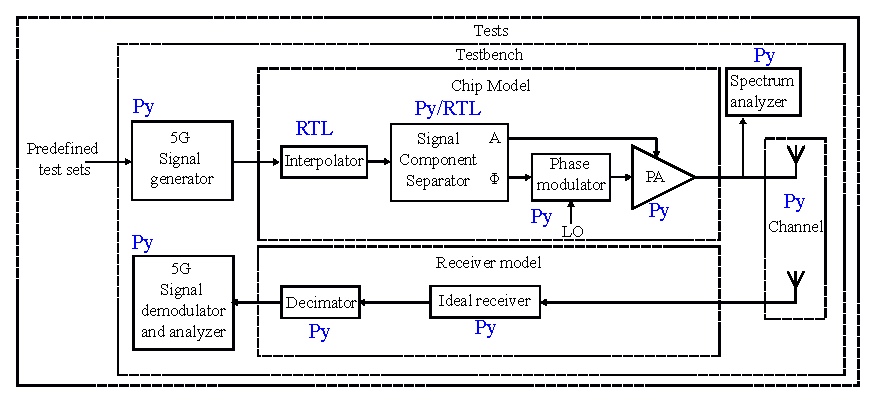
\includegraphics[width=0.5\textwidth]{Pics/outphasing_model_interp.eps}
    \end{center}
    \begin{figure}
        \subfloat[Interpolator (HW, EVM)]{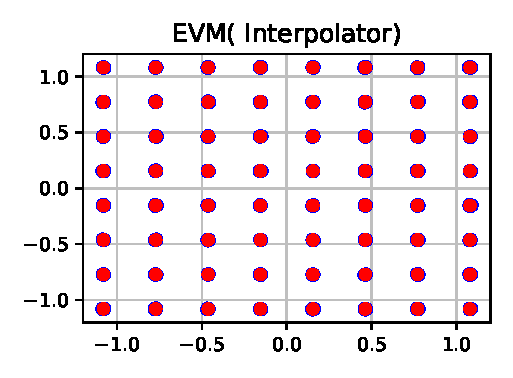
\includegraphics[width=0.4\textwidth]{Pics/evm_interp_v4.eps}}\qquad
        \subfloat[Interpolator (HW,
        ACLR)]{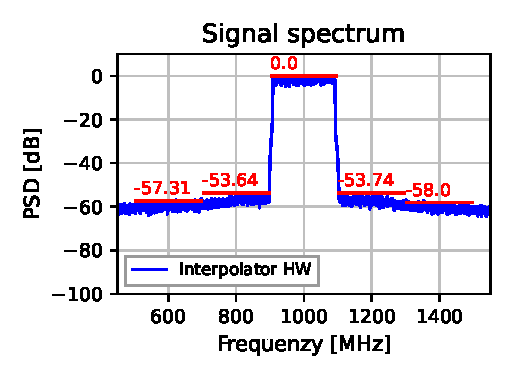
\includegraphics[width=0.4\textwidth]{Pics/interp_hw_ACLR_v4.eps}}
    \end{figure}
    \begin{itemize}
        \item EVM : $0.338\%$
        \item ACLR: $-53.64, -53.74$ dB
    \end{itemize}

\end{frame}
%%%%%%%%%%%%%%%%%%%%%%%%%%%%%%%%%%%%%%%%%%%%
\begin{frame}[t]
    \frametitle{Interpolator hardware EVM and ACLR}
    \begin{center}
        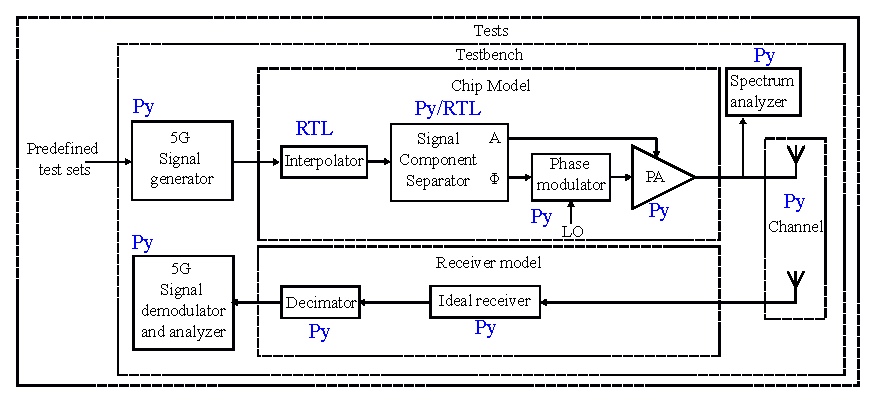
\includegraphics[width=0.5\textwidth]{Pics/outphasing_model_interp.eps}
    \end{center}
    \begin{figure}
        \begin{center}
            \subfloat[Interpolator (HW, EVM)]{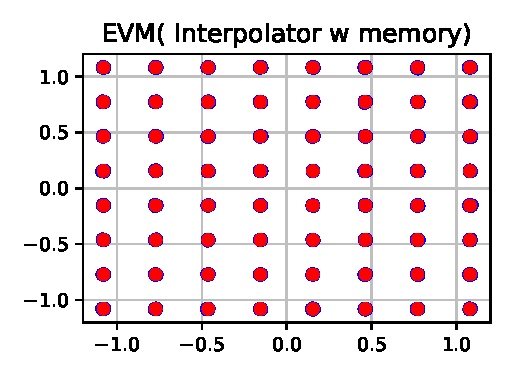
\includegraphics[width=0.4\textwidth]{./Pics/evm_interp_v4wmem.eps}}\qquad
            \subfloat[Interpolator (HW, ACLR)]{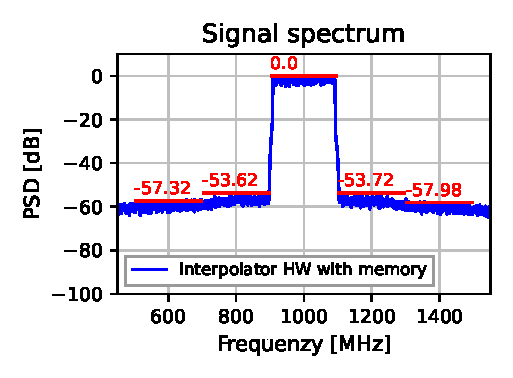
\includegraphics[width=0.4\textwidth]{./Pics/interp_hw_ACLR_v4wmem.eps}}
        \end{center}
    \end{figure}
    \begin{itemize}
        \item EVM : $0.339\%$
        \item ACLR: $ -53.62, -53.71$ dB
    \end{itemize}
\end{frame}

%%%%%%%%%%%%%%%%%%%%%%%%%%%%%%%%%%%%%%%%%%
\begin{frame}[t]
    \frametitle{SCS 6-bit resolution EVM}
    \begin{center}
        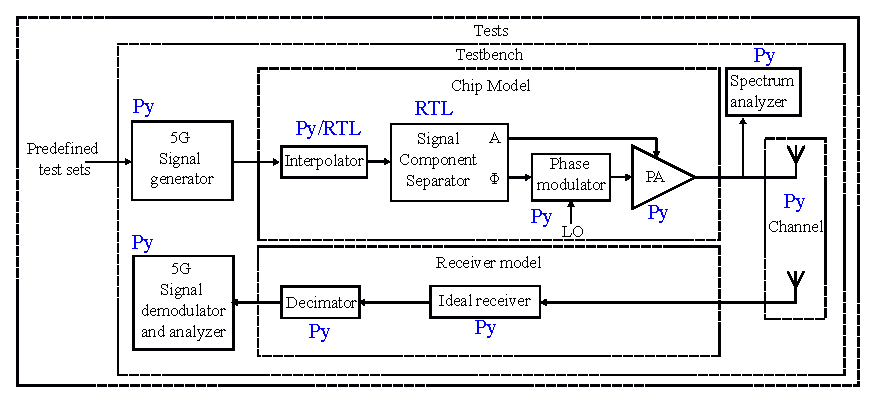
\includegraphics[width=0.5\textwidth]{Pics/outphasing_model_scs.eps}
    \end{center}
    \begin{figure}
        \subfloat[EVM, SCS RTL simulation)]{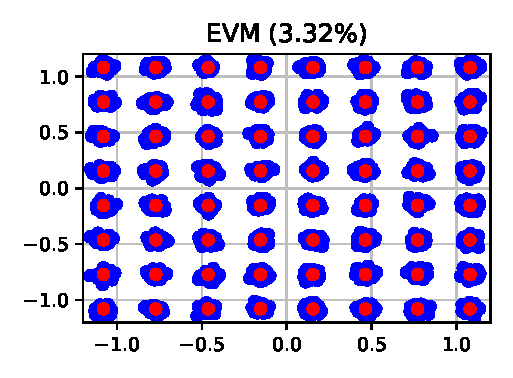
\includegraphics[height=4cm,width=5cm]{./Pics/evm_6bit_scswmem.eps}}\qquad
        \subfloat[ACLR, SCS RTL simulation)]{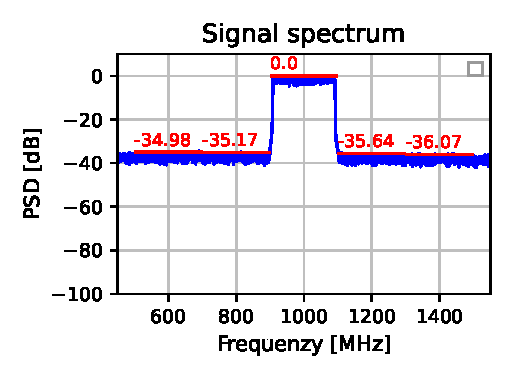
\includegraphics[height=4cm,width=5cm]{./Pics/scswmem_res6_ACLR.eps}}
    \end{figure}
\end{frame}

%%%%%%%%%%%%%%%%%%%%%%%%%%%%%%%%%%%%%%%%%%%%
\begin{frame}[t]
    \frametitle{SCS 10-bit resolution hardware EVM and ACLR }
    \begin{center}
        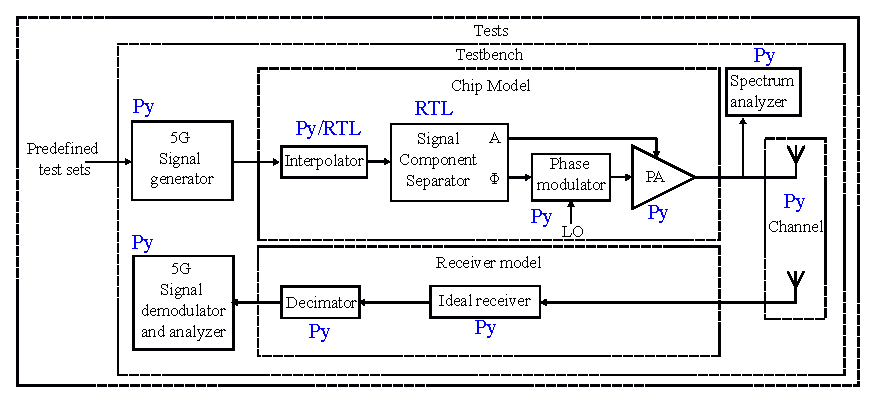
\includegraphics[width=0.5\textwidth]{Pics/outphasing_model_scs.eps}
    \end{center}
    \begin{figure}
        \begin{center}
            \subfloat[EVM SCS RTL simulation]{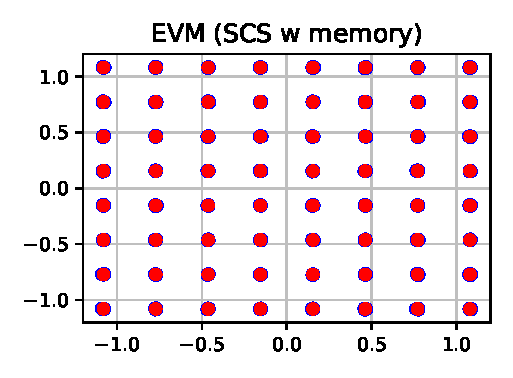
\includegraphics[width=0.4\textwidth]{./Pics/evm_10bit_scs_v6wmem.eps}}\qquad
            \subfloat[ACLR SCS RTL simulation]{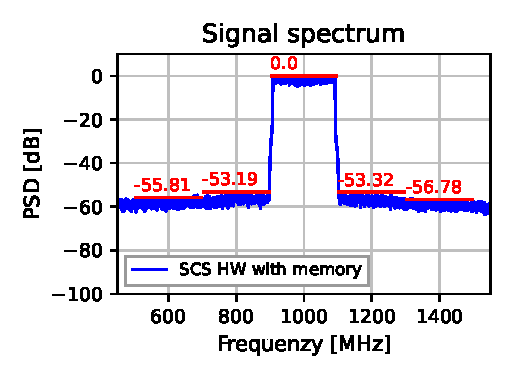
\includegraphics[width=0.4\textwidth]{./Pics/scs_10b_ACLR_v6wmem.eps}}
        \end{center}
    \end{figure}
    \begin{itemize}
        \item EVM: $0.336\%$
        \item ACLR: $-53.18, -53.31$ dB
    \end{itemize}
\end{frame}


\sectiontitle[Example 6: A-Core RISC-V processor chip]
%%%%%%%%%%%%%%%%%%%%%%%%%%%%%%%%%%%%%%%%%%%
\renewcommand{\sectionname}{A-Core RISC-V processor chip}
\subsection*{\sectionname}
\begin{frame}[c]
    \frametitle{\sectionname}
    \begin{itemize}
        \item SoC built with ACoreBase
        \item AXI4-Lite on-chip interconnect
        \item Memory mapped peripherals
            \begin{itemize}
                \item Random Access Memory (RAM)
                \item Read-only access to instruction memory (ProgMem)
                \item General Purpose Input/Output (GPIO)
                \item Custom accelerator IP
            \end{itemize}
    \end{itemize}
        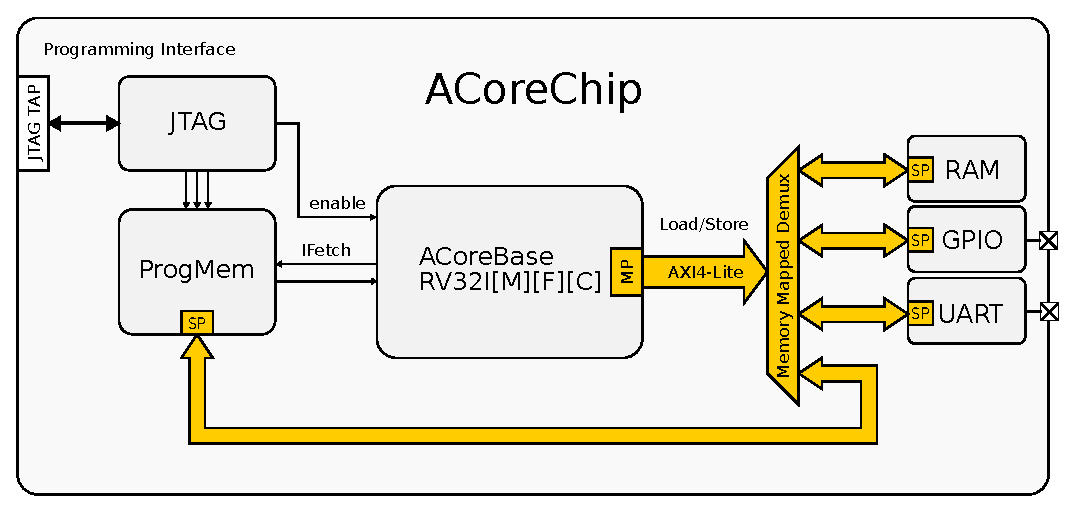
\includegraphics[width=.8\textwidth]{./Pics/acorechip.eps}
\end{frame}

%%%%%%%%%%%%%%%%%%%%%%%%%%%%%%%%%%%%%%%%%%
\renewcommand{\sectionname}{A-Core chip TheSydeKick verification}
\subsection*{\sectionname}
\begin{frame}[c]
    \frametitle{A-Core chip verification }
    \begin{block}{A-Core test setup}
        \begin{center}
            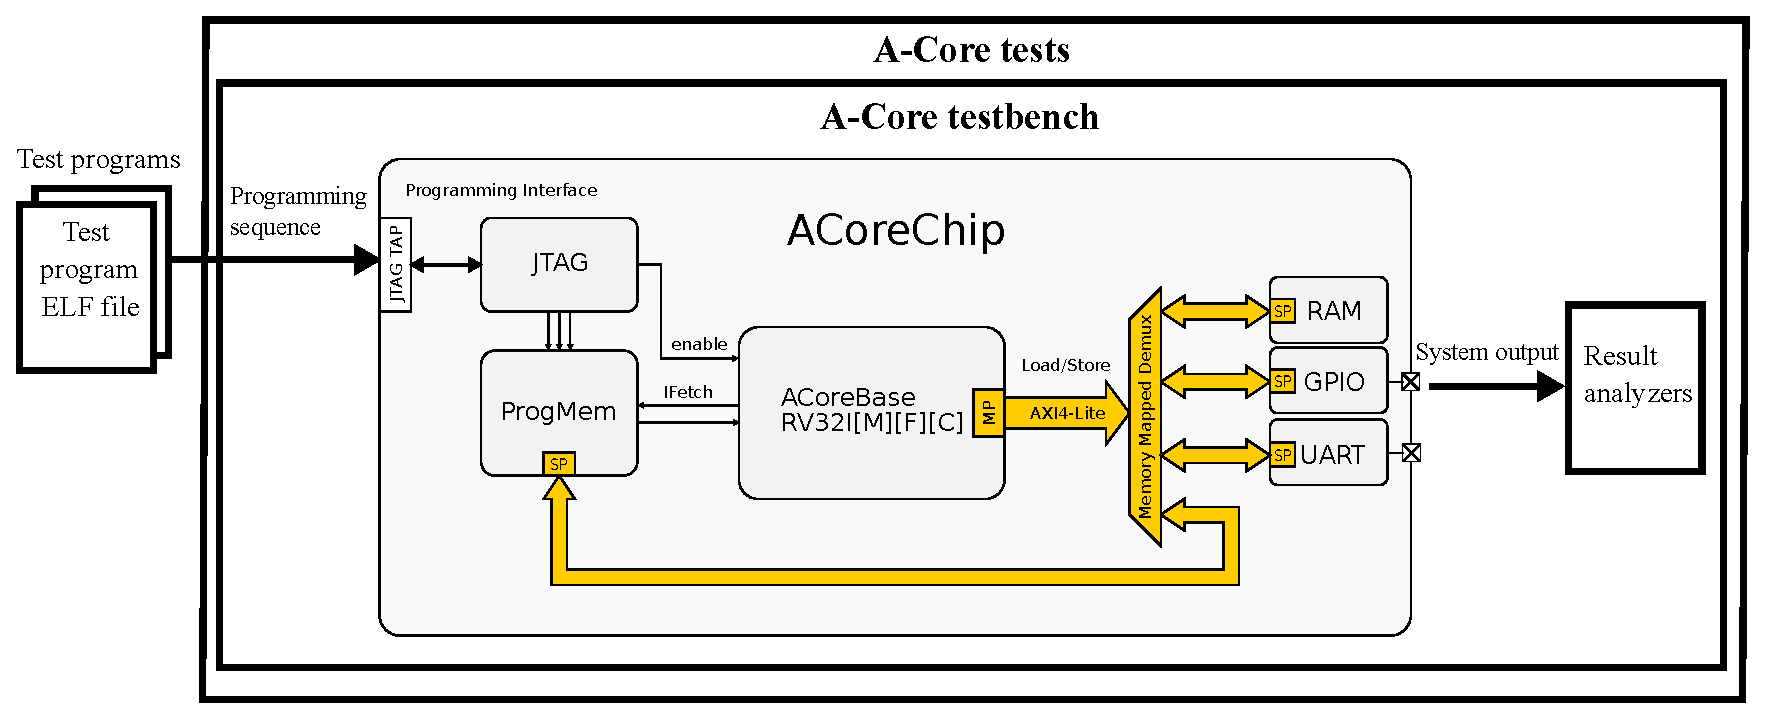
\includegraphics[width=\textwidth]{./Pics/A-Core_testsetup.eps}
        \end{center}
    \end{block}
\end{frame}

%%%%%%%%%%%%%%%%%%%%%%%%%%%%%%%%%%%%%%%%%%
\renewcommand{\sectionname}{TheSyDeKick simulations}
\subsection*{\sectionname}
\begin{frame}[t]
    \frametitle{\sectionname}
    \begin{itemize}
        \item For system-level simulations
        \item TheSyDeKick automates the following verification tasks
        \begin{itemize}
            \item Generate a simulation test vector
            \begin{itemize}
                \item JTAG programming waveform from ELF file
                \item Chip control signals (e.g. core enable)
            \end{itemize}
            \item Generate a verilog testbench
            \item Invoke a digital simulator (ModelSim)
        \end{itemize}
    \end{itemize}
    \begin{center}
        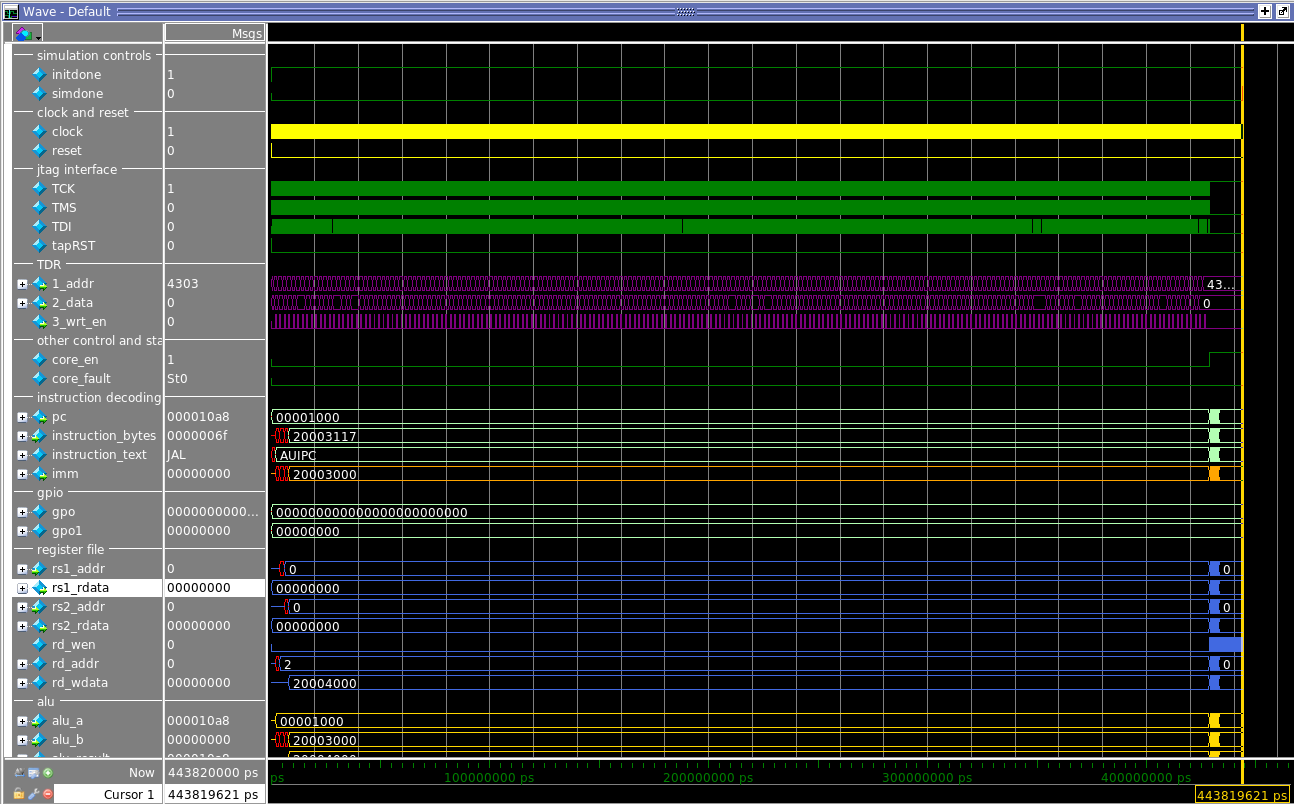
\includegraphics[width=0.65\linewidth]{./Pics/prog_sequence.png}
    \end{center}
\end{frame}

%%%%%%%%%%%%%%%%%%%%%%%%%%%%%%%%%%%%%%%%%%
\renewcommand{\sectionname}{ACoreChip Entity}
\subsection*{\sectionname}
\begin{frame}[c,fragile]
    \frametitle{\sectionname}
    \begin{itemize}
        \item Represents a simulatable model of ACoreChip
        \item Submodules
        \begin{itemize}
            \item ACoreChip Chisel generator \verb|chisel/|
        \end{itemize}
    \end{itemize}
    \begin{block}{A-Core test setup}
        \begin{center}
            \includegraphics[width=0.5\textwidth]{./Pics/A-Core_testsetup.eps}
        \end{center}
    \end{block}
\end{frame}

%%%%%%%%%%%%%%%%%%%%%%%%%%%%%%%%%%%%%%%%%%
\renewcommand{\sectionname}{ACoreTestbenches}
\subsection*{\sectionname}
\begin{frame}[t,fragile]
    \frametitle{\sectionname}
    \begin{itemize}
        \item \verb|ACoreTestbenches| instance represents a test bench
            configuration.
        \item Testbench configuration is selected with appropriate
            \verb|define*|
            method
        \begin{itemize}
            \item For example, \verb|define_acorechip_sim_testbench(**kwargs)|
                configures test-bench as a acorechip simulation.
            \item Software, jtag config., etc. are provided as keyword
                arguments to \verb|define*|
        \end{itemize}
    \end{itemize}
    \begin{block}{A-Core test setup}
        \begin{center}
            \includegraphics[width=0.5\textwidth]{./Pics/A-Core_testsetup.eps}
        \end{center}
    \end{block}
\end{frame}

%%%%%%%%%%%%%%%%%%%%%%%%%%%%%%%%%%%%%%%%%%
\renewcommand{\sectionname}{ACoreTestbenches}
\subsection*{\sectionname}
\begin{frame}[t,fragile]
    \frametitle{\sectionname}
    \begin{itemize}
        \item A testbench configuration is a general combination of entities
            and related configuration for representing a unique test setup.
        \item The simulation testbench has two options: The SyDeKick and cocotb
        \begin{itemize}
            \item The SyDeKick uses its own structures to generate the Verilog testbench, IO's and run with modelsim
            \item Cocotb runs a cocotb test - can be used to create interactive debug environments in the future
        \end{itemize}
    \end{itemize}
    \begin{block}{A-Core test setup}
        \begin{center}
            \includegraphics[width=0.5\textwidth]{./Pics/A-Core_testsetup.eps}
        \end{center}
    \end{block}
\end{frame}

%%%%%%%%%%%%%%%%%%%%%%%%%%%%%%%%%%%%%%%%%%
\renewcommand{\sectionname}{ACoreTests}
\subsection*{\sectionname}
\begin{frame}[t,fragile]
    \frametitle{\sectionname}
    \begin{itemize}
        \item \verb|ACoreTests| contains different concrete parameterizations
            of \verb|ACoreTestbenches| and their dependencies:
        \begin{itemize}
            \item Test software live under \verb|sw/|
            \item Simulation specific do-files live under
                \verb|interactive_control_files/modelsim|
        \end{itemize}
        \item Each test is defined as a method under \verb|ACoreTests| class.
        \item For example, \verb|sim_f_tests| configures a testbench with
            \begin{itemize}
                \item F-extension enabled
                \item test program for f-extension
            \end{itemize}
    \end{itemize}
    \begin{block}{A-Core test setup}
        \begin{center}
            \includegraphics[width=0.5\textwidth]{./Pics/A-Core_testsetup.eps}
        \end{center}
    \end{block}
\end{frame}

%%%%%%%%%%%%%%%%%%%%%%%%%%%%%%%%%%%%%%%%%%
\renewcommand{\sectionname}{ACoreTests}
\subsection*{\sectionname}
\begin{frame}[t,fragile]
    \frametitle{\sectionname}
    \begin{itemize}
        \item The test to be executed is selected with a command line
            argument. For example, \verb|$ ./configure && make sim test_target=sim_f_tests|
            runs the simulation defined as \verb|sim_f_tests|
        \item The simulator option can be selected with \verb|simulator| argument for make, 
            for example \verb|$ make sim test_target=sim_f_tests simulator=cocotb|
    \end{itemize}
    \begin{block}{A-Core test setup}
        \begin{center}
            \includegraphics[width=0.5\textwidth]{./Pics/A-Core_testsetup.eps}
        \end{center}
    \end{block}
\end{frame}

%%%%%%%%%%%%%%%%%%%%%%%%%%%%%%%%%%%%%%%%%%%%%%%%%%%%%%%%%%%%%%%%%%%%%%%%%%
\sectiontitle[Example 7: EM field simulations]

%%%%%%%%%%%%%%%%%%%%%%%%%%%%%%%%%%%%%%%%%%
\renewcommand{\sectionname}{Layout preparation}
\subsection*{\sectionname}
\begin{frame}[c]
    \frametitle{\sectionname}
    \begin{itemize}
        \item Preparations: Constructing the layout from TheSyDeKick with
            Berkeley Analog Generator.
        \item Active development of BAG2 currently ongoing at
            \emph{https://gitlab.com/mosaic\_group/mosaic\_BAG}
    \end{itemize}
    \begin{minipage}[t]{0.48\textwidth}
        \vskip 0pt
        \begin{block}{BAG workflow}
            \begin{center}
                \includegraphics[width=\textwidth]{./Pics/bag_workflow}
            \end{center}
        \end{block}
    \end{minipage}\hfill
    \begin{minipage}[t]{0.48\textwidth}
        \vskip 0pt
        \begin{block}{TheSyDeKick project structure}
            \begin{center}
                \includegraphics[width=0.4\textwidth]{./Pics/sdk_dirtree_v2}
                \includegraphics[width=0.58\textwidth]{./Pics/sdk_structure_v3}
            \end{center}
        \end{block}
    \end{minipage}
\end{frame}
%%%%%%%%%%%%%%%%%%%%%%%%%%%%%%%%%%%%%%%%%%
\renewcommand{\sectionname}{Transformer design flow diagram}
\subsection*{\sectionname}
\begin{frame}[c]
    \frametitle{\sectionname}
    \begin{block}{Design flow}
        \begin{center}
            \includegraphics[width=0.8\linewidth]{./Pics/inductor_flow_diagram.pdf}
        \end{center}
    \end{block}
\end{frame}
%%%%%%%%%%%%%%%%%%%%%%%%%%%%%%%%%%%%%%%%%%
\renewcommand{\sectionname}{Transformer structures}
\subsection*{\sectionname}
\begin{frame}[c]
    \frametitle{\sectionname}
    \begin{itemize}
        \item Parameters: Wire width, transformer diameter.
    \end{itemize}
    \begin{minipage}[t]{0.48\textwidth}
        \vskip 0pt
        \begin{block}{A stacked transformer}
            \begin{center}
                \includegraphics[width=\textwidth]{./Pics/stacked_TF_3D_view_white_background.png}
            \end{center}
        \end{block}
    \end{minipage}\hfill
    \begin{minipage}[t]{0.48\textwidth}
        \vskip 0pt
        \begin{block}{An Interwound transformer}
            \begin{center}
                \includegraphics[width=0.85\textwidth]{./Pics/int_TF_3D_white_background_2.png}
            \end{center}
        \end{block}
    \end{minipage}
\end{frame}

%%%%%%%%%%%%%%%%%%%%%%%%%%%%%%%%%%%%%%%%%%
\renewcommand{\sectionname}{Transfer functions}
\subsection*{\sectionname}
\begin{frame}[c]
    \frametitle{\sectionname}
    \begin{minipage}[t]{0.48\textwidth}
        \vskip 0pt
        \begin{block}{Transfer function of a stacked transformer}
            \begin{center}
                \includegraphics[width=\textwidth]{./Pics/diff_S21_stacked_TF_diam_width_sweep_3.pdf}
            \end{center}
        \end{block}
    \end{minipage}\hfill
    \begin{minipage}[t]{0.48\textwidth}
        \vskip 0pt
        \begin{block}{Transfer function of an interwound transformer}
            \begin{center}
                \includegraphics[width=\textwidth]{./Pics/diff_S21_int_TF_diam_width_sweep_3.pdf}
            \end{center}
        \end{block}
    \end{minipage}
\end{frame}

%%%%%%%%%%%%%%%%%%%%%%%%%%%%%%%%%%%%%%%%%%
\renewcommand{\sectionname}{Insertion loss}
\subsection*{\sectionname}
\begin{frame}[c]
    \frametitle{\sectionname}
    \begin{minipage}[t]{0.48\textwidth}
        \vskip 0pt
        \begin{block}{Insertion loss of a stacked transformer}
            \begin{center}
                \includegraphics[width=\textwidth]{./Pics/diff_S21_stacked_TF_3Dbar_diam_width_sweep_2.pdf}
            \end{center}
        \end{block}
    \end{minipage}\hfill
    \begin{minipage}[t]{0.48\textwidth}
        \vskip 0pt
        \begin{block}{Insertion loss of an interwound transformer}
            \begin{center}
                \includegraphics[width=\textwidth]{./Pics/diff_S21_int_TF_3Dbar_diam_width_sweep_4.pdf}
            \end{center}
        \end{block}
    \end{minipage}
\end{frame}
%%%%%%%%%%%%%%%%%%%%%%%%%%%%%%%%%%%%%%%%%%%
%\renewcommand{\sectionname}{ECD BAG project structure}
%\subsection*{\sectionname}
%\begin{frame}[t]
%    \frametitle{\sectionname}
%    \begin{block}{ECD BAG project structure}
%    \begin{minipage}[t]{0.3\textwidth}
%    \parbox{\textwidth}{
%        \dirtree{% 
%            .1 virtuoso\_BAG/.
%            .2 BAG\_technology\_definition/.
%            .2 BAG\_framework/.
%            .2 BAG2\_EC\_TEMPLATES/.
%            .2 bag\_ecd/.
%            .2 amplifier\_bag/.
%            .3 amplifier\_bag/.
%            .4 \_\_init\_\_.py.
%            .4 schematic.py.
%            .4 layout.py.
%            .4 doc/.
%        }
%    }
%    \end{minipage}
%    \end{block}
%\end{frame}
%
%%%%%%%%%%%%%%%%%%%%%%%%%%%%%%%%%%%%%%%%%%%
%\renewcommand{\sectionname}{ECD TheSyDeKick-BAG project structure}
%\subsection*{\sectionname}
%\begin{frame}[t]
%    \frametitle{\sectionname}
%    \begin{block}{TheSyDeKick-BAG project structure}
%    \begin{minipage}[t]{0.41\textwidth}
%    \parbox{\textwidth}{
%        \dirtree{% 
%            .1 thesydekick\_project/.
%            .2 Entities/.
%            .3 thesdk/.
%            .3 spice/.
%            .3 rtl/.
%            .3 amplifier/.
%            .4 amplifier/.
%            .5 \_\_init\_\_.py.
%            .5 schematic.py.
%            .5 layout.py.
%            .4 spice/.
%            .4 Simulations/.
%            .4 doc/.
%        }
%    }
%    \end{minipage}
%    \begin{minipage}[t]{0.41\textwidth}
%    \parbox{\textwidth}{
%        \dirtree{% 
%            .1 virtuoso\_BAG/.
%            .2 BAG\_technology\_definition/.
%            .2 BAG\_framework/.
%            .2 BAG2\_EC\_TEMPLATES/.
%            .2 bag\_ecd/.
%            .2 amplifier/.
%            .3 amplifier/.
%            .4 \_\_init\_\_.py.
%            .4 schematic.py.
%            .4 layout.py.
%            .3 spice/.
%            .3 Simulations/.
%            .3 doc/.
%        }
%    }
%    \end{minipage}
%    \end{block}
%\end{frame}

%%% Additions by Santeri

%%%%%%%%%%%%%%%%%%%%%%%%%%%%%%%%%%%%%%%%%%%%%%%%%%%%%%%%%%%%%%%%%%%%%%%%%%
\sectiontitle[Conclusion and acknowledgements]
%%%%%%%%%%%%%%%%%%%%%%%%%%%%%%%%%%%%%%%%%%%%%%%%%%%%%%%%%%%%%%%%%%%%%%%%%%%%%
\renewcommand{\sectionname}{Conclusion}
\subsection*{\sectionname}
\begin{frame}[t]
    \frametitle{\sectionname}
    \begin{itemize}
        \item Modular design environment through well defined IO boundaries and
            \emph{Entity} definitions.
        \item Open Source
        \item Automates repetitive verification tasks and provides means for programmatic
            verification with various simulators
        \item Support for measurement equipment under development.
        \item \emph{Enables} co-development by multiple designers using various
            verification tools.
        \item \emph{Enabled by} utilization of programming methodology and
            version control in hardware design context.
    \end{itemize}
\end{frame}

%%%%%%%%%%%%%%%%%%%%%%%%%%%%%%%%%%%%%%%%%%%%%%%%%%%%%%%%%%%%%%%%%%%%%%%%%%%%%
\renewcommand{\sectionname}{Acknowledgement}
\subsection*{\sectionname}
\begin{frame}[t]
    \frametitle{\sectionname}
    \begin{itemize}

        \item TheSyDeKick framework has been initiated during 2017-2019 under Marie
            Sklodowska-Curie project \emph{ADVANTAG5}, in collaboration with Aalto
            University and University of California, Berkeley. (See licences,
                \emph{https://github.com/TheSystemDevelopmentKit/thesdk}
            )
        \item Since the end of  \emph{ADVANTAG5} 2019, Lot of valuable
            development work has been carried out by several students of Aalto
            University, Finland.  
    \end{itemize} 

    \vfill

    \tiny{This project has received funding from the European Union’s
        Horizon 2020 research and innovation programme under the Marie
        Sklodowska-Curie grant agreement No 704947. Results reflects only
        the author's view and the European Comissions's Research Executive
        Agency Agency is not responsible for any use that may be made of
    the information it contains. }
\end{frame}

\end{document}
